% Created 2021-03-12 Fri 15:11
\documentclass[titlepage]{article}
\usepackage[utf8]{inputenc}
\usepackage[T1]{fontenc}
\usepackage{graphicx}
\usepackage{grffile}
\usepackage{longtable}
\usepackage{wrapfig}
\usepackage{rotating}
\usepackage[normalem]{ulem}
\usepackage{amsmath}
\usepackage{textcomp}
\usepackage{amssymb}
\usepackage{capt-of}
\usepackage{hyperref}
\usepackage{minted}
\usepackage{mathptmx}
\author{Xiong ChenYu(U1521516C) \\
EEE \\
}
\date{Apr. 8, 2018 \\
}
\title{
\includegraphics[width=\textwidth]{img/NTU.png} \\
[2\baselineskip] Assignment ON \\
EE4478 Digital video processing\\
Tutorial 2-12 \\
[3\baselineskip]}
\hypersetup{
 pdfauthor={Xiong ChenYu(U1521516C) \\
EEE \\
},
 pdftitle={
\includegraphics[width=\textwidth]{img/NTU.png} \\
[2\baselineskip] Assignment ON \\
EE4478 Digital video processing\\
Tutorial 2-12 \\
[3\baselineskip]},
 pdfkeywords={},
 pdfsubject={},
 pdfcreator={Emacs 27.1 (Org mode 9.5)}, 
 pdflang={English}}
\begin{document}

\maketitle
\tableofcontents

\listoflistings

\newpage


\section{Assignment 2 Halffman Code}
\label{sec:org5f80d0c}
\subsection{Question 1}
\label{sec:org2d265ba}

   To generate halfman code first is to sort combile the 2 items with lowest possibilites and resort. Until the table only have 2
items left.

\begin{table}[htbp]
\caption{1st round of sort}
\centering
\begin{tabular}{lr}
Symbol & Probalility\\
\hline
C & 0.05\\
A & 0.1\\
F & 0.12\\
D & 0.18\\
B & 0.2\\
E & 0.35\\
\end{tabular}
\end{table}

\begin{table}[htbp]
\caption{combile \& 2nd round of sort}
\centering
\begin{tabular}{lr}
Symbol & Probalility\\
\hline
F & 0.12\\
AC & 0.15\\
D & 0.18\\
B & 0.2\\
E & 0.35\\
\end{tabular}
\end{table}

\begin{table}[htbp]
\caption{\label{fig:label}combile \& 3rd round of sort}
\centering
\begin{tabular}{lr}
Symbol & Probalility\\
\hline
D & 0.18\\
B & 0.2\\
ACF & 0.27\\
E & 0.35\\
\end{tabular}
\end{table}


\begin{table}[htbp]
\caption{\label{fig:label}combile \& 4th round of sort}
\centering
\begin{tabular}{lr}
Symbol & Probalility\\
\hline
ACF & 0.27\\
E & 0.35\\
BD & 0.38\\
\end{tabular}
\end{table}

\begin{table}[htbp]
\caption{\label{fig:label}combile \& 5th round of sort}
\centering
\begin{tabular}{lr}
Symbol & Probalility\\
\hline
BD & 0.38\\
ACFE & 0.62\\
\end{tabular}
\end{table}

Then I can use the table above to generate halfman tree, I will use the 0 for the low probalities. And 1 for the high probalities.

\begin{figure}[htbp]
\centering
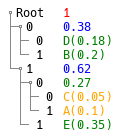
\includegraphics[width=5cm]{img/btree1.png}
\caption{\label{fig:1}Tutorial 2.1}
\end{figure}

After generate the halfman tree, I can generate the halfman code by go through the path

\begin{table}[htbp]
\caption{Halfman code table}
\centering
\begin{tabular}{lr}
Symbol & Code\\
\hline
C & 1010\\
A & 1011\\
F & 100\\
D & 00\\
B & 01\\
E & 11\\
\end{tabular}
\end{table}


\newpage

\subsection{Question 2}
\label{sec:orgdd45b35}

   To generate halfman code first is to sort combile the 2 items with lowest possibilites and resort. Until the table only have 2
items left.

\begin{table}[htbp]
\caption{1st round of sort}
\centering
\begin{tabular}{lr}
Symbol & Probalility\\
\hline
A & 0.04\\
B & 0.1\\
C & 0.11\\
D & 0.15\\
G & 0.18\\
E & 0.2\\
F & 0.22\\
\end{tabular}
\end{table}


\begin{table}[htbp]
\caption{combile \& 2nd round of sort}
\centering
\begin{tabular}{lr}
Symbol & Probalility\\
\hline
C & 0.11\\
AB & 0.14\\
D & 0.15\\
G & 0.18\\
E & 0.2\\
F & 0.22\\
\end{tabular}
\end{table}

\begin{table}[htbp]
\caption{\label{fig:label}combile \& 3rd round of sort}
\centering
\begin{tabular}{lr}
Symbol & Probalility\\
\hline
D & 0.15\\
G & 0.18\\
E & 0.2\\
F & 0.22\\
ABC & 0.25\\
\end{tabular}
\end{table}

\begin{table}[htbp]
\caption{\label{fig:label}combile \& 4th round of sort}
\centering
\begin{tabular}{lr}
Symbol & Probalility\\
\hline
E & 0.2\\
F & 0.22\\
ABC & 0.25\\
DG & 0.33\\
\end{tabular}
\end{table}

\begin{table}[htbp]
\caption{\label{fig:label}combile \& 5th round of sort}
\centering
\begin{tabular}{lr}
Symbol & Probalility\\
\hline
ABC & 0.25\\
DG & 0.33\\
EF & 0.42\\
\end{tabular}
\end{table}

\begin{table}[htbp]
\caption{\label{fig:label}combile \& 6th round of sort}
\centering
\begin{tabular}{lr}
Symbol & Probalility\\
\hline
EF & 0.42\\
ABCDG & 0.58\\
\end{tabular}
\end{table}

Then I can use the table above to generate halfman tree, I will use the 0 for the low probalities. And 1 for the high probalities.

\begin{figure}[htbp]
\centering
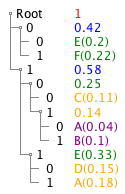
\includegraphics[width=5cm]{img/btree2.png}
\caption{\label{fig:2}Tutorial 2.2}
\end{figure}

After generate the halfman tree, I can generate the halfman code by go through the path

\begin{table}[htbp]
\caption{Halfman code table}
\centering
\begin{tabular}{lr}
Symbol & Code\\
\hline
A & 1010\\
B & 1011\\
C & 100\\
D & 110\\
G & 111\\
E & 00\\
F & 01\\
\end{tabular}
\end{table}

\newpage

\section{Assignment 3 Arithmetic Coding}
\label{sec:org3c0589c}

My matric card is shown below in \hyperref[fig:3]{Figure 3} So my matric number is U1521516C my last 8 character is 1521561C.

\begin{figure}[htbp]
\centering
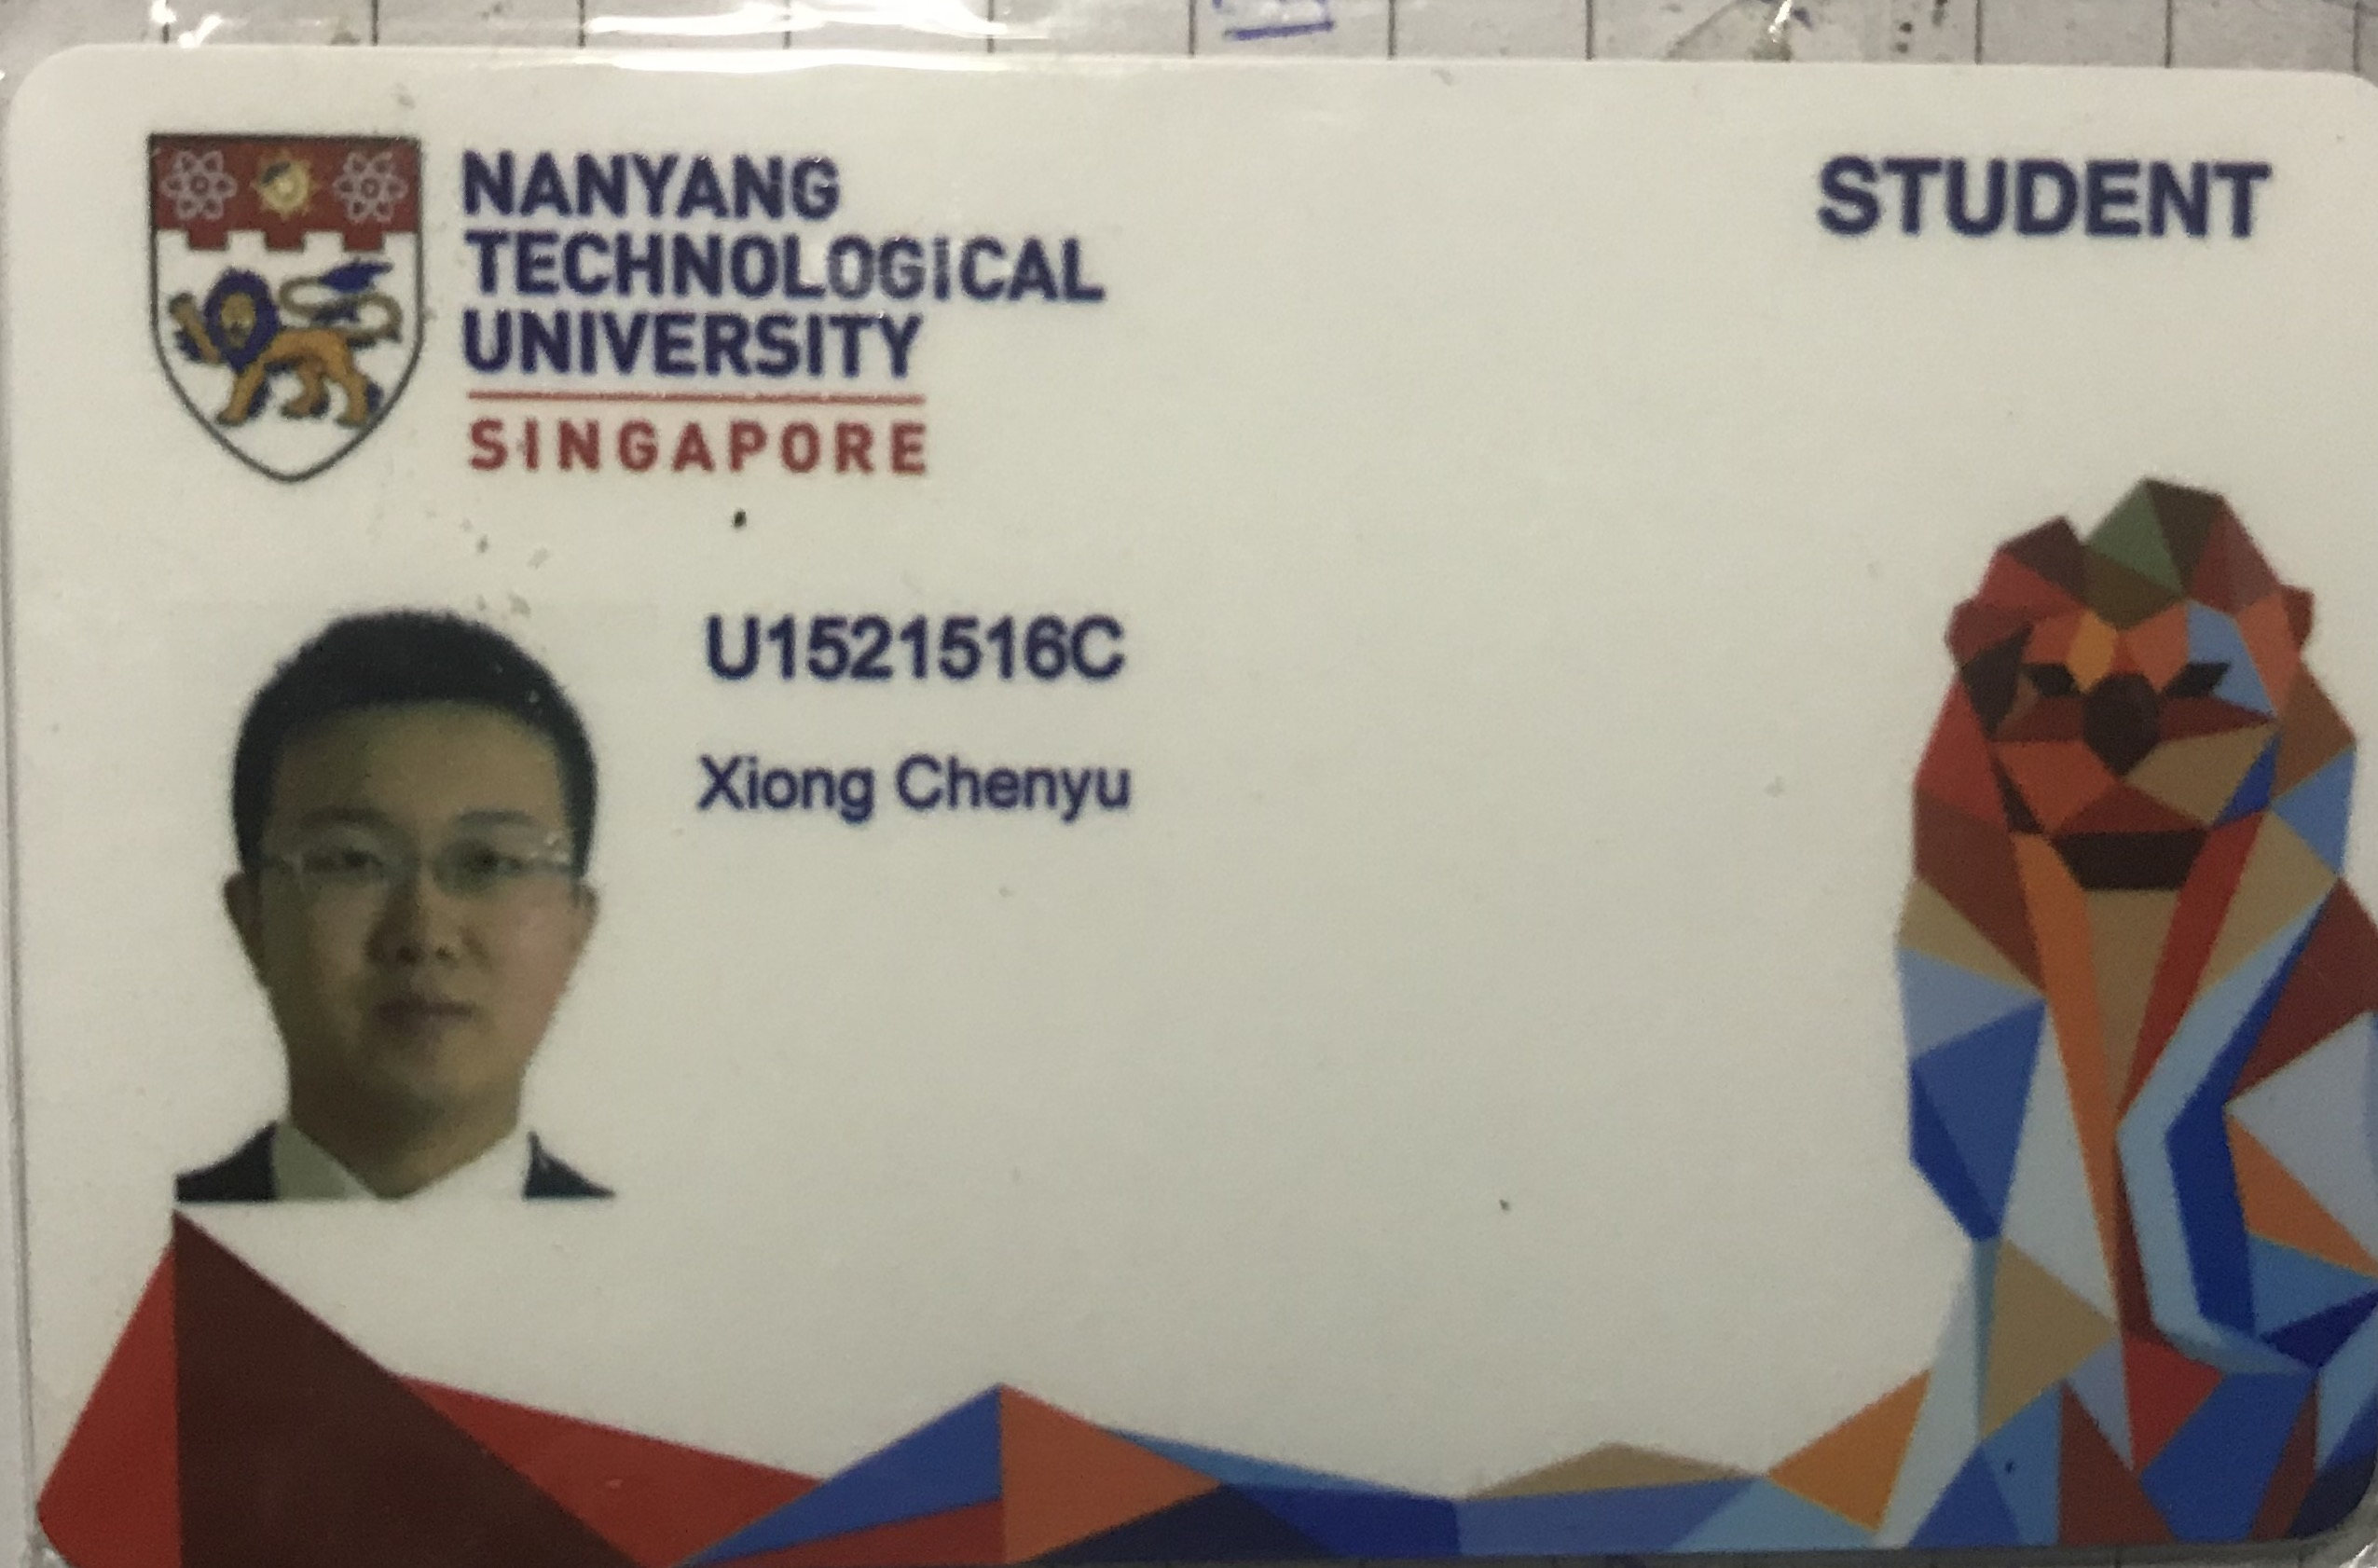
\includegraphics[width=5cm]{./img/mat.jpg}
\caption{\label{fig:3}Matriculation Card}
\end{figure}

\begin{center}
\begin{tabular}{rr}
Symbol & Frequet Number\\
\hline
1 & 3\\
2 & 1\\
5 & 2\\
6 & 1\\
C & 1\\
\end{tabular}
\end{center}

SO each range will be \(\frac{1}{8} = 0.125\), So we can gererate arthmetic table

\begin{center}
\begin{tabular}{rlrrr}
Symbol & Probability & Interval  Low & Interval   High & Interval\\
\hline
1 & \(\frac{3}{8}\) & 0 & 0.375 & 0.375\\
2 & \(\frac{1}{8}\) & 0.375 & 0.5 & 0.125\\
5 & \(\frac{1}{4}\) & 0.5 & 0.75 & 0.25\\
6 & \(\frac{1}{8}\) & 0.75 & 0.875 & 0.125\\
C & \(\frac{1}{8}\) & 0.875 & 1 & 0.125\\
\end{tabular}
\end{center}

\begin{center}
\begin{tabular}{rll}
New Char & Low Value & High Value\\
\hline
1 & 0 & 0.375\\
5 & \(0 + (0.375 - 0) \times 0.5 =  0.1875\) & \(0 + (0.375 -0) \times 0.75 = 0.2813\)\\
2 & \(0.1875 + (0.2813 - 0.1875) \times 0.375 = 0.2227\) & \(0.1875 + (0.2813 - 0.1875) \times 0.5 = 0.2344\)\\
1 & \(0.2227 + (0.2344 - 0.2227) \times 0 = 0.2227\) & \(0.2227 + (0.2344 - 0.2227) \times 0.375 = 0.2271\)\\
5 & \(0.2227 + (0.2271-0.2227) \times 0.5 = 0.2249\) & \(0.2227 + (0.2271-0.2227) \times 0.75 = 0.2260\)\\
1 & \(0.2249 + (0.2260 - 0.2249) \times 0 = 0.2249\) & \(0.2249 + (0.2260 - 0.2249) \times 0.375 = 0.2253\)\\
6 & \(0.2249 + (0.2253 - 0.2249) \times 0.75 = 0.2252\) & \(0.2249 + (0.2253 - 0.2249) \times 0.875 = 0.22525\)\\
C & \(0.2252 + (0.22525 - 0.2252) \times 0.875 = 0.22524375\) & \(0.2252 + (0.22525 - 0.2252) \times 1 = 0.22525\)\\
\end{tabular}
\end{center}

\begin{center}
\begin{tabular}{rrrrr}
Decoded Number & Output Symbol & Low & High & Interval\\
\hline
0.22524375 & 1 & 0 & 0.375 & 0.375\\
0.60065 & 5 & 0.5 & 0.75 & 0.25\\
0.4022 & 2 & 0.375 & 0.5 & 0.125\\
0.2177 & 1 & 0 & 0.375 & 0.375\\
0.5806 & 5 & 0.5 & 0.75 & 0.25\\
0.3223 & 1 & 0 & 0.375 & 0.375\\
0.8594 & 6 & 0.75 & 0.875 & 0.125\\
0.8750 & C & 0.875 & 1 & 0.125\\
\end{tabular}
\end{center}


\newpage

\section{Assignment 4 Discrete Cosine Transform (DCT)}
\label{sec:org553b917}

$$A = \begin{Bmatrix}
      \frac{1}{2}cos(0) & \frac{1}{2}cos(0) & \frac{1}{2}cos(0) & \frac{1}{2}cos(0) \\
     \sqrt{\frac{1}{2}}cos(\frac{\pi}{8}) & \sqrt{\frac{1}{2}}cos(\frac{3\pi}{8}) & \sqrt{\frac{1}{2}}cos(\frac{5\pi}{8}) & \sqrt{\frac{1}{2}}cos(\frac{7\pi}{8}) \\
      \sqrt{\frac{1}{2}}cos(\frac{2\pi}{8}) & \sqrt{\frac{1}{2}}cos(\frac{6\pi}{8}) & \sqrt{\frac{1}{2}}cos(\frac{10\pi}{8}) & \sqrt{\frac{1}{2}}cos(\frac{14\pi}{8}) \\
      \sqrt{\frac{1}{2}}cos(\frac{3\pi}{8}) & \sqrt{\frac{1}{2}}cos(\frac{9\pi}{8}) & \sqrt{\frac{1}{2}}cos(\frac{15\pi}{8}) & \sqrt{\frac{1}{2}}cos(\frac{21\pi}{8})
   \end{Bmatrix}$$

$$X =\begin{Bmatrix}
      5 & 5 & 10 & 10 \\
      5 & 10 & 10 & 10 \\
      1 & 10 & 10 & 10 \\
      1 & 1 & 5 & 10
   \end{Bmatrix}$$

$$A^T = \begin{Bmatrix}
      \frac{1}{2}cos(0) &  \sqrt{\frac{1}{2}}cos(\frac{\pi}{8})& \sqrt{\frac{1}{2}}cos(\frac{2\pi}{8}) &  \sqrt{\frac{1}{2}}cos(\frac{3\pi}{8})\\
      \frac{1}{2}cos(0)& \sqrt{\frac{1}{2}}cos(\frac{3\pi}{8}) & \sqrt{\frac{1}{2}}cos(\frac{6\pi}{8})  & \sqrt{\frac{1}{2}}cos(\frac{9\pi}{8}) \\
       \frac{1}{2}cos(0)&  \sqrt{\frac{1}{2}}cos(\frac{5\pi}{8})& \sqrt{\frac{1}{2}}cos(\frac{10\pi}{8}) & \sqrt{\frac{1}{2}}cos(\frac{15\pi}{8})  \\
       \frac{1}{2}cos(0)&  \sqrt{\frac{1}{2}}cos(\frac{7\pi}{8})& \sqrt{\frac{1}{2}}cos(\frac{14\pi}{8})& \sqrt{\frac{1}{2}}cos(\frac{21\pi}{8})
   \end{Bmatrix}$$

$$Y' = A \times X  =\begin{Bmatrix}
      6 & 13 & 17.5 & 20 \\
      3.6955 & 2.6131 & 3.2664 & 0 \\
      0 & -7 & -2.5 & 0 \\
      -1.5307 & 1.0823 & 1.325 & 0
   \end{Bmatrix}$$


$$Y = Y' \times X  =\begin{Bmatrix}
      28.25 & -10.36 & -2.25 & -0.8486 \\
      4.7875 & 2.22374 & -1.092 & 1.4268 \\
      -4.75 & -1.2177 & 4.75 & 2.9398 \\
      0.45 & -1.073 & -1.983 & -0.237
   \end{Bmatrix}$$


\section{Assignment 5 Discrete Cosine Transform (DCT)}
\label{sec:org7318c39}

\begin{minted}[]{matlab}
clear all;
close all;
clc;
raw_input_img=imread('lena512c.jpg');
redChannel = dct2(raw_input_img(:, :, 1));
greenChannel = dct2(raw_input_img(:, :, 2));
blueChannel = dct2(raw_input_img(:, :, 3));
input_img = cat(3, redChannel, greenChannel, blueChannel);
QP=10;
quantized_img=round(input_img./QP);
rec_img=quantized_img.*QP;
n_img = cat(3,idct2(rec_img(:, :, 1)),idct2(rec_img(:, :, 2)),idct2(rec_img(:, :, 3)));
error= double(raw_input_img) - n_img;
subplot(1,4,1);
imshow(raw_input_img);
title('Original image');
subplot(1,4,2);
imshow(uint8(n_img));
title(['Reconstructed image (QP=' num2str(QP) ')']);
subplot(1,4,3);
imshow(error);
title('quantization error')
\end{minted}

The output shown in below and I find that the higher the quant level the quality of the imgae will drop and more color appear in error.
\begin{center}
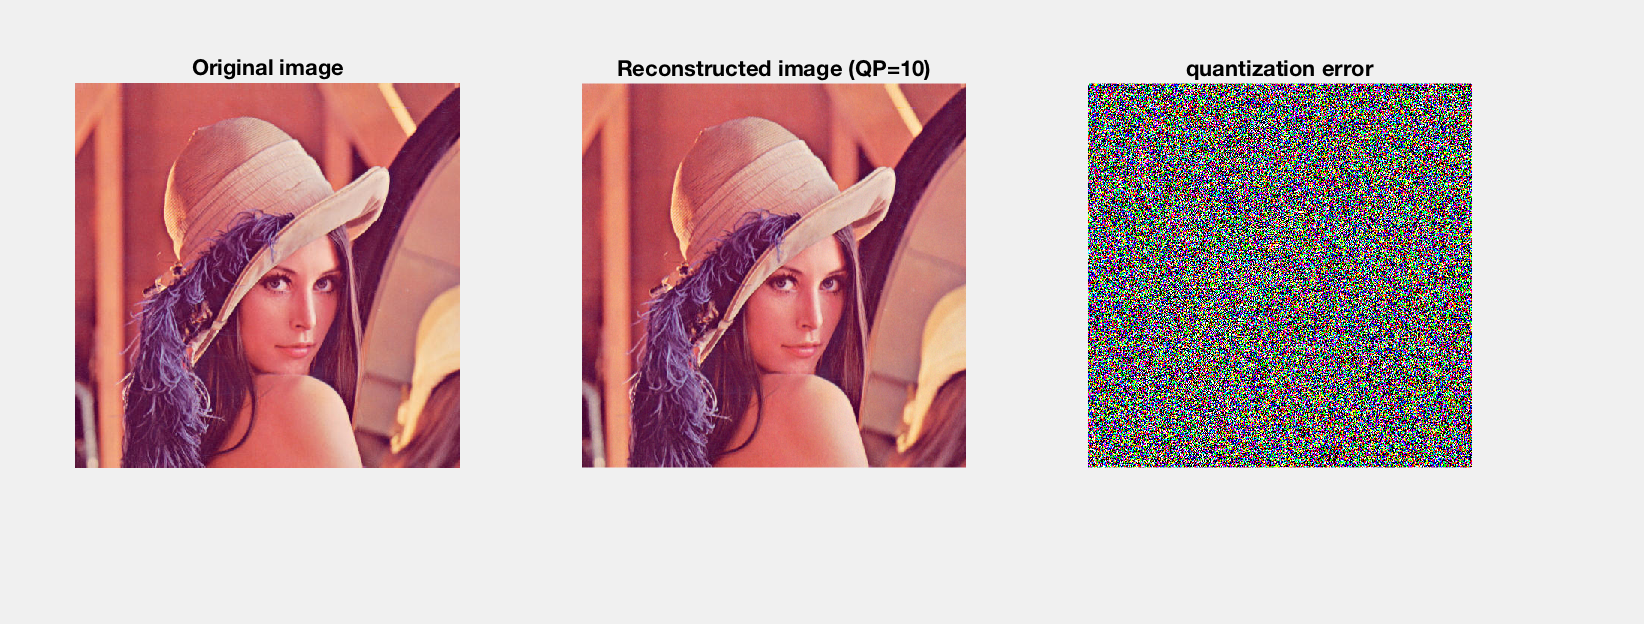
\includegraphics[width=.9\linewidth]{./img/quant.png}
\end{center}

\section{Assignment 6 Zig-Zag Scan}
\label{sec:org26fb97a}
\subsection{Question a}
\label{sec:orgf1daac1}
My name is xiongchenyu so the matric will be

$$in =\begin{matrix}
      x & i & o & n \\
      g & c & h & e \\
      n & y & u & x \\
      i & o & n & g
   \end{matrix}$$

The input matric in matlab will be [120 105 111 110;103 99 104 101;110 121 117 120;105 111 110 103]

out =

120   105   103   110    99   111   110   104   121   105   111   117   101   120   110   103

\subsection{Question b}
\label{sec:orgcd88d1b}

in = [4    -1     0     0; 1     0     0     0  ;-1    0     1     0; 0     0     0     0]

out = 4	-1	1	-1	0	0	0	0	0	0	0	1	0	0	0	0


\subsection{Question c}
\label{sec:orga21da1e}

I just change the input to 8 * 8 I think the origin code will support artitury shape to do the zigzag.

in =[

 7    -1     0    -2    -1     1     0    -1;
 1     0     0     0     0     0     0     0;
 0     0     0     0     0     0     0     0;
 1     0     0     0     0     0     0     0;
-1     0     0     0     1     0     0     1;
 0     0     0     0     0     0     0     0;
 0     0     0     0     0     0     0     0;
 0     0     0     0    -1     0     0     0]

out =

Columns 1 through 22

7    -1     1     0     0     0    -2     0     0     1    -1     0     0     0    -1     1     0     0     0     0     0     0

Columns 23 through 44

0     0     0     0     0     0    -1     0     0     0     0     0     0     0     0     0     0     1     0     0     0     0

Columns 45 through 64

0     0     0     0     0     0     0     0     0     0     1     0     0    -1     0     0     0     0     0     0


\section{Assignment 7 Run-Level Coding (RLC)}
\label{sec:org316de68}

\subsection{Question a}
\label{sec:org75669b4}
\begin{minted}[]{matlab}

x =  round(200 * rand(1,40));
x(x>40) = 0;

array = [1 5 2 1 5 1 6 zeros(1,28)]
\end{minted}


x =

Columns 1 through 21

0     0     0     0     0     7    28     0     0     0     0     0     5     9     0     0     0     0     0     0     0

Columns 22 through 40

0     0    30     5     0    30    18     0    35    32     0     0     0     0    14     0     0     0     0

\subsection{Question b}
\label{sec:org24b29b9}
\begin{minted}[]{matlab}

sizeOfSequence = 40
y = round(35 * rand(1,sizeOfSequence));
for i = 1:length(y)
    y(i) = array(y(i));
end

\end{minted}

y =

Columns 1 through 21

0     1     1     0     0     0     0     0     0     0     0     0     0     0     0     0     0     0     1     0     0

Columns 22 through 40

0     0     0     0     0     0     1     0     0     0     0     5     1     0     0     2     0     6     0


\section{Assignment 8 JPEG / MPEG Intra frame encoding}
\label{sec:org1933cc4}

\begin{minted}[]{matlab}
A=imread('photo.jpg');
[Height,Width,Depth]=size(A);
\end{minted}

\begin{figure}[htbp]
\centering
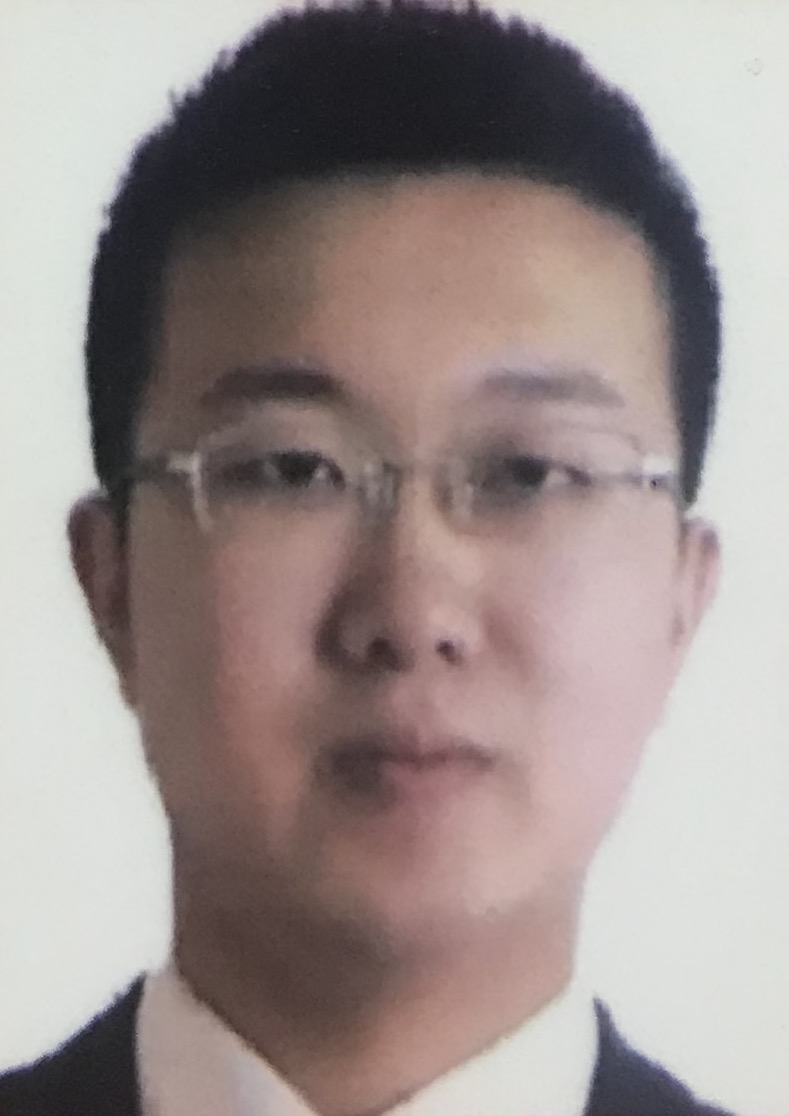
\includegraphics[width=.9\linewidth]{./img/photo.jpg}
\caption{\label{fig:label}Orgion}
\end{figure}

\begin{center}
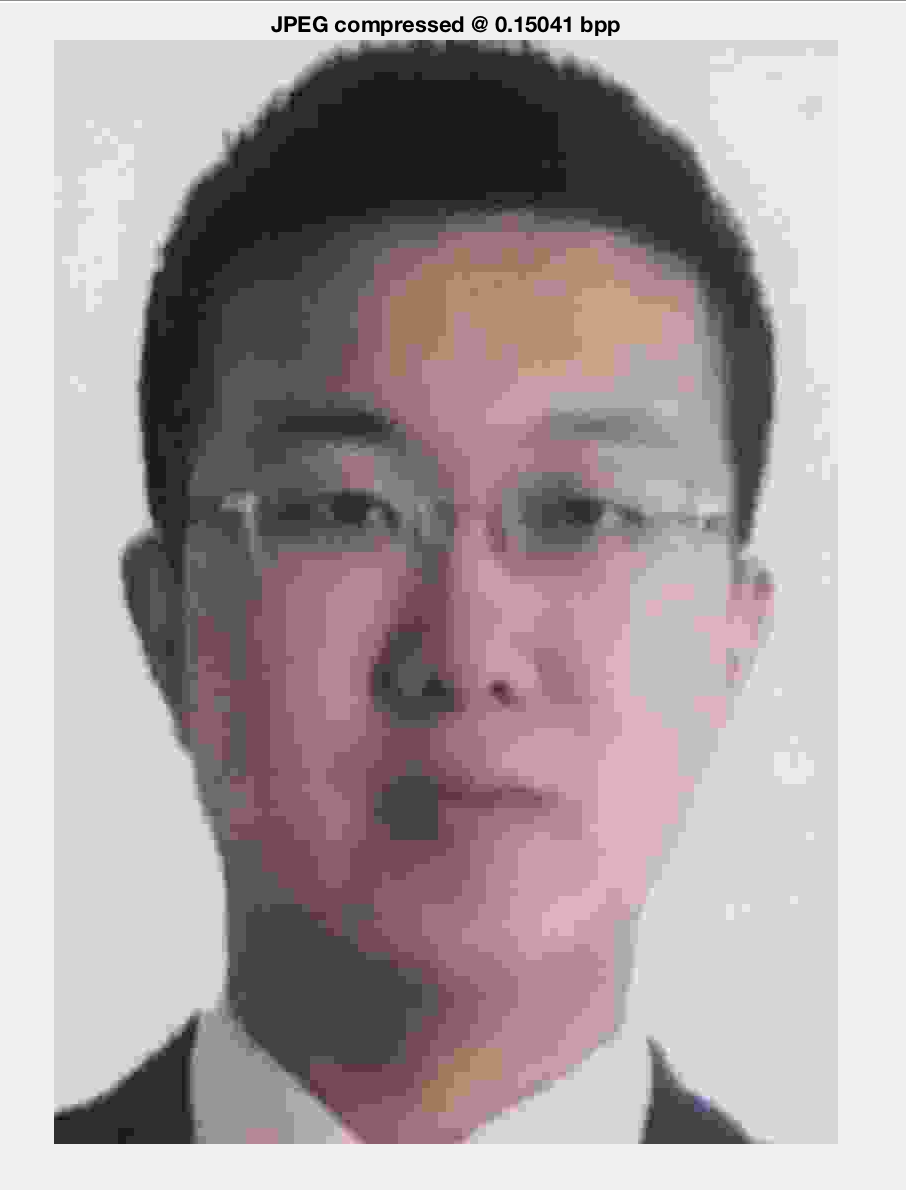
\includegraphics[width=.9\linewidth]{./img/p15_9.png}
\end{center}

\begin{center}
\begin{tabular}{ll}
Type & Value\\
\hline
Oscale & 9\\
PSNR & 31.61dB\\
SNR(Cb) & 34.99dB\\
PSNR(Cr) & 34.24dB\\
\end{tabular}
\end{center}

\begin{center}
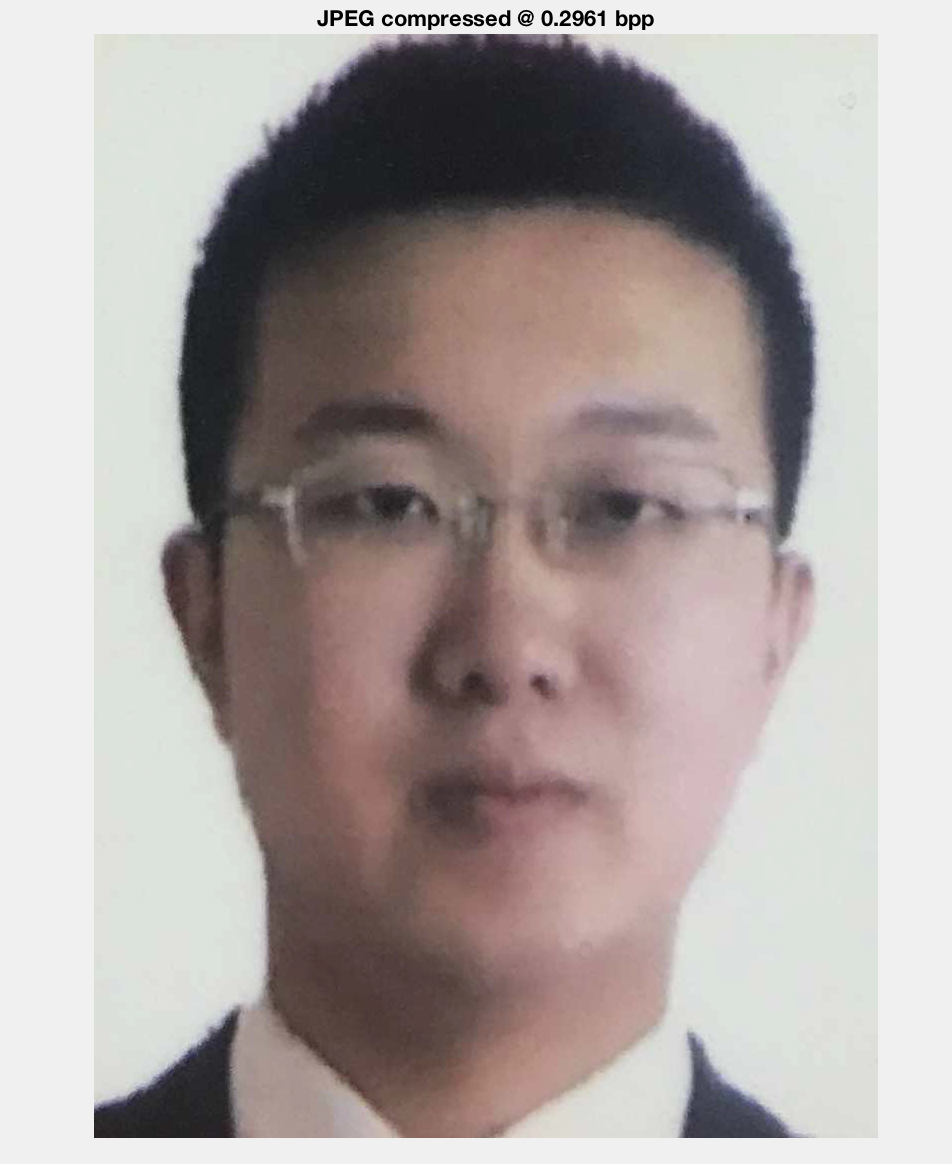
\includegraphics[width=.9\linewidth]{./img/p3_83.png}
\end{center}

\begin{center}
\begin{tabular}{ll}
type & value\\
\hline
oscale & 0.83\\
psnr & 45.41db\\
snr(cb) & 50.49db\\
psnr(cr) & 50.25db\\
\end{tabular}
\end{center}

\begin{center}
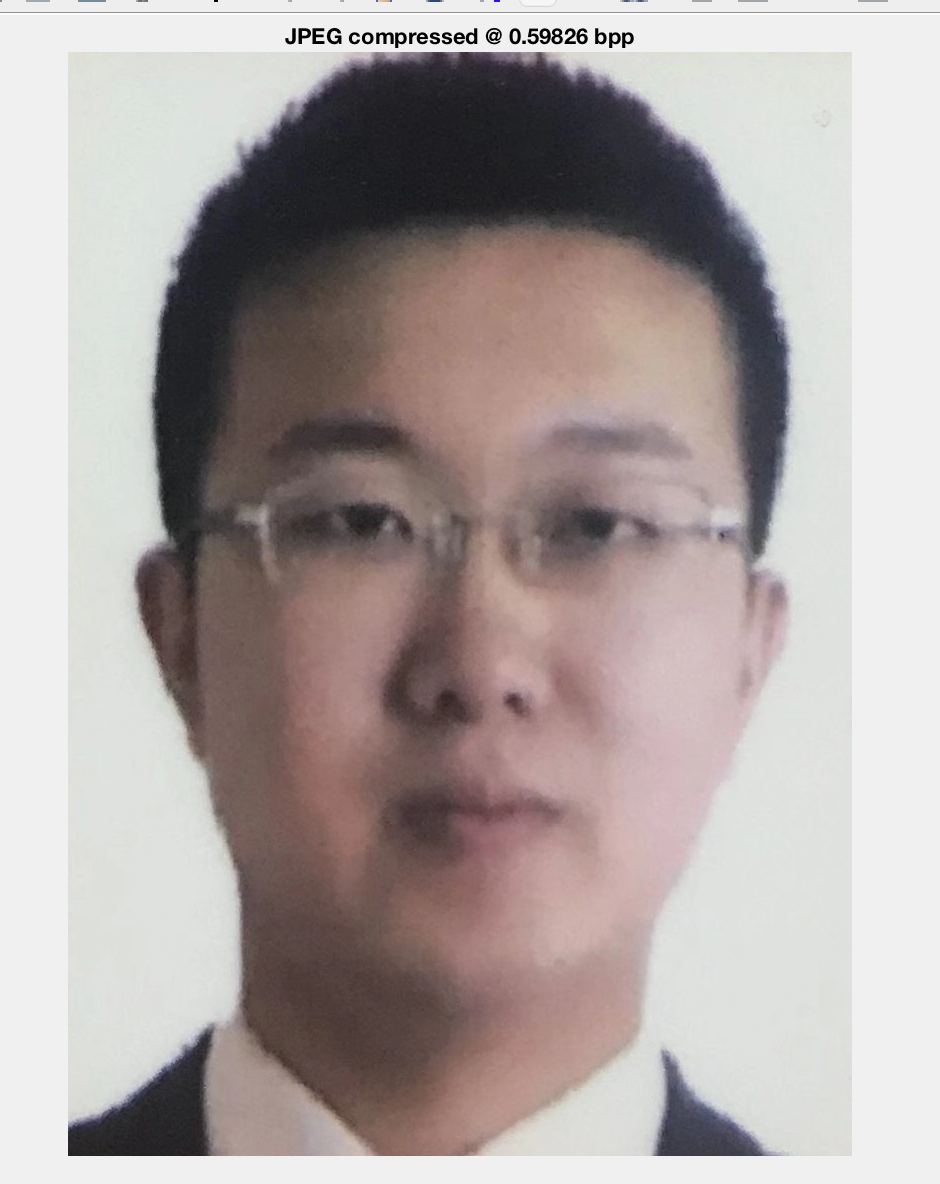
\includegraphics[width=.9\linewidth]{./img/p6_332.png}
\end{center}

\begin{center}
\begin{tabular}{ll}
Type & Value\\
\hline
Oscale & 0.332\\
PSNR & 49.43dB\\
SNR(Cb) & 54.69dB\\
PSNR(Cr) & 54.64dB\\
\end{tabular}
\end{center}




\section{Assignment 9 Motion estimation}
\label{sec:org58c0bb0}
\subsection{Apply quantization error on MC prediction error}
\label{sec:org366c6f5}

\subsection{Question a}
\label{sec:orgf50108c}

\subsection{Question b}
\label{sec:org963d6bd}
\subsection{Question c}
\label{sec:org3cf9e8e}


\section{Assignment 10}
\label{sec:org2622ac6}

\begin{enumerate}
\item Uncomment \% A=transpose(A);  line 26
\item Uncomment \% B=transpose(B);  line 63
\item The image size normaliztion is incorrect.
\end{enumerate}
\begin{minted}[]{matlab}
% Make image size divisible by 16
[X,Y] = size(A);
if mod(X,16)~=0
    Height = floor(X/16)*16;
else
    Height = X;
end
if mod(Y,16)~=0
    Width = floor(Y/16)*16;
else
    Width = Y;
end
\end{minted}

change to 8 as

\begin{minted}[]{matlab}
% Make image size divisible by 8
[X,Y] = size(A);
if mod(X,8)~=0
    Height = floor(X/16)*16;
else
    Height = X;
end
if mod(Y,8)~=0
    Width = floor(Y/16)*16;
else
    Width = Y;
end

\end{minted}

line 23

\begin{enumerate}
\item change inFile1='table\textsubscript{40.raw}'; to 'table\textsubscript{39.raw}' line 23
\item change F = int16(41:43); to F = int16(40:43); line 50
\item change legend('MC','No MC', 0) to legend('MC','No MC', 'best') line 114
\item change legend('MC','No MC', 0) to legend('MC','No MC', 'best') line 118
\end{enumerate}



\section{Assignment 11 Stereo Imaging}
\label{sec:org23cdbc8}

Original : D = round(Y2\{nf\}/2);  \%adjust depth factor '2'

Modify To : D = round(Y2\{nf\}/5);
\end{document}
